\section{Referencial Teórico}

Apresentar o texto referente a base conceitual. A base conceitual é caracterizada pela referência de obras que tratam do assunto do presente trabalho permitindo o embasamento teórico e metodológico a partir da análise das mais recentes obras científicas que tratam do assunto.

Para citar figuras, o processo é semelhante ao de tabelas, como na \autoref{fig:fig1}.  Citações bibliográficas são feitas de maneira semelhante, porém deve ser inserido o identificador da referência contida no arquivo .bib, como em \cite{lange1998programming}. Citações também estão disponíveis na forma \textcite{lange1998programming} ou, para uma página específica, como é feito na citação direta abaixo. Equações também podem ser inseridas, conforme é feito a seguir. O código para inserí-las pode ser gerado no site \href{https://www.codecogs.com/latex/eqneditor.php?lang=pt-br}{\textbf{CodeCogs}}.

% Exemplo de inserção de equação
\[\Delta =b^{2}-4ac\]
\[x=\frac{-b\pm\sqrt{\Delta }}{2a}\]

% Exemplo de inserção de figura
\begin{figure}[htbp]
    \centering
    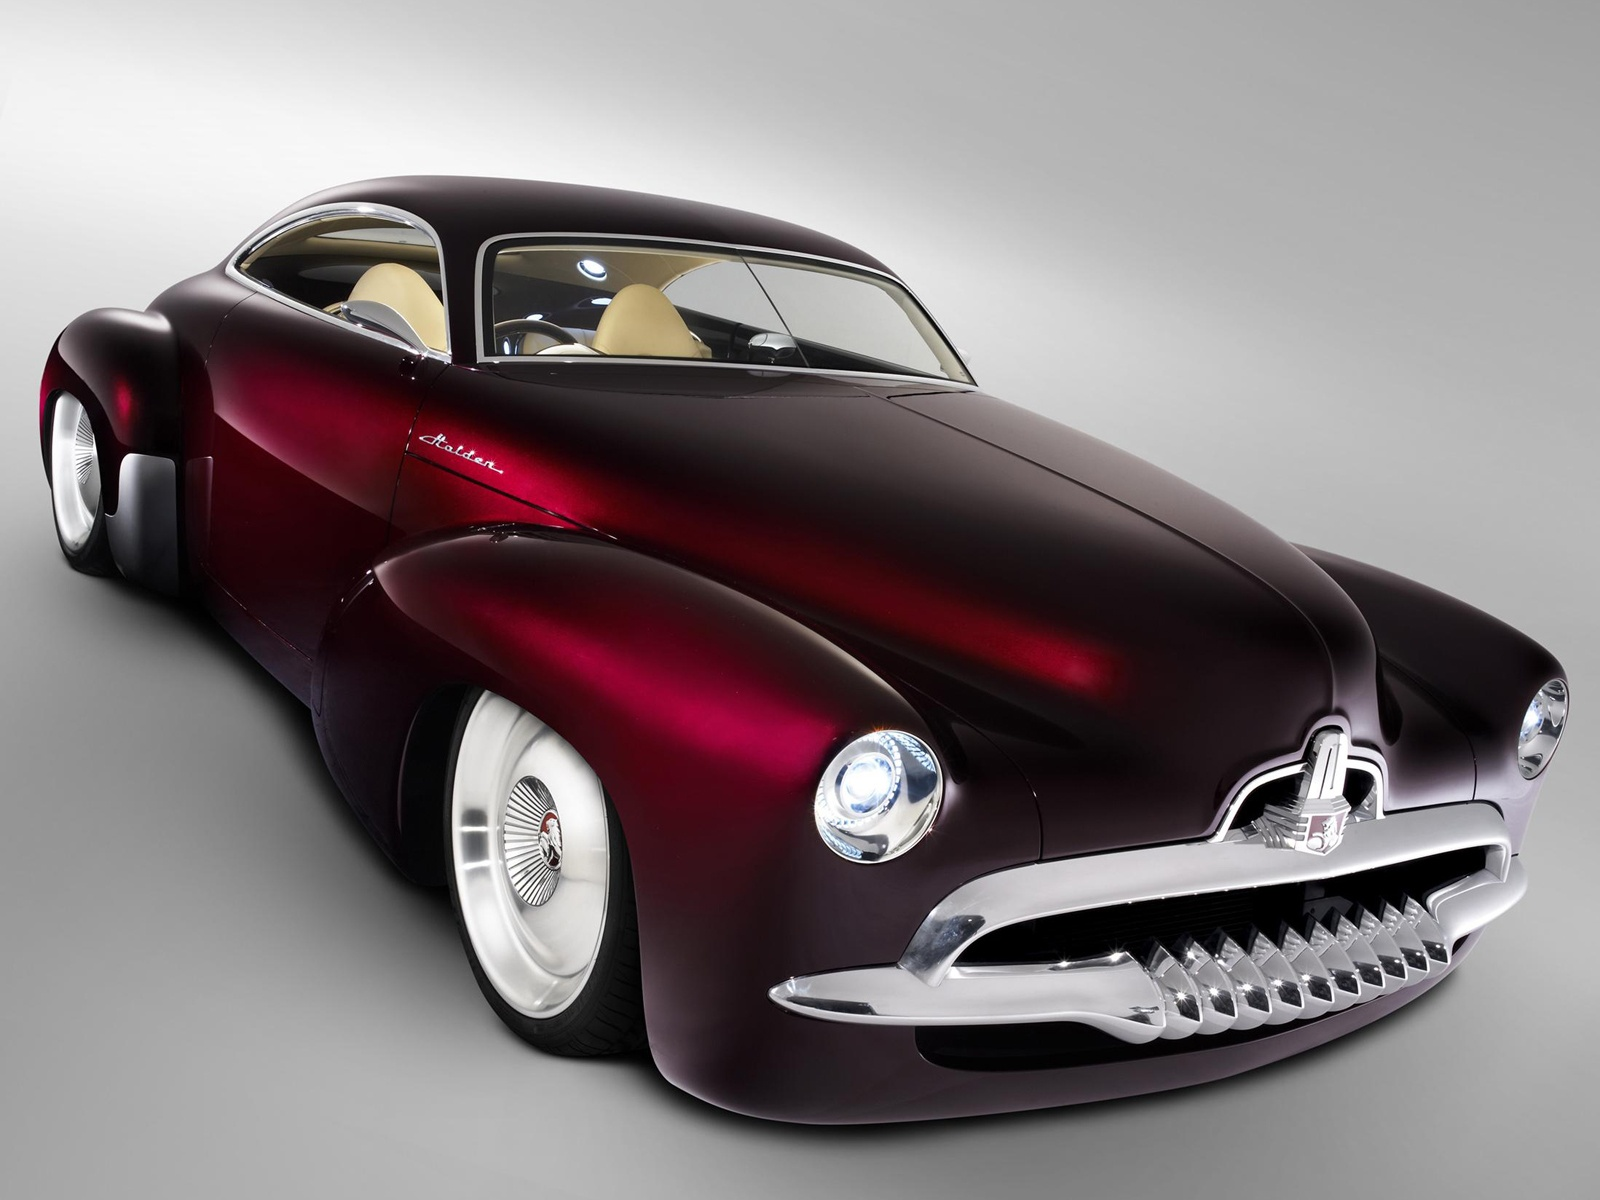
\includegraphics[width=7cm]{anexos/fig1.jpg} % URI da figura
    \caption{
    % Legenda da figura
    Carro vermelho
    }
    \label{fig:fig1} % Tag para referência
\end{figure}

No caso do uso de citação direta longa (que possuem mais de 3 linhas) deve-se utilizar fonte arial tamanho 11, recuo a esquerda de 4 cm, com alinhamento do texto justificado e espaçamento de parágrafo em 0 pt antes e 0 pt depois.

% Exemplo de citação
\begingroup
\leftskip4cm
\small{

\noindent
Todo o texto deve ser justificado, com o recuo de primeira linha do parágrafo em 1,25 cm, exceto em citação direta com mais de três linhas, a qual deve possuir recuo de 4 cm, partindo da margem esquerda. \textcite[p. 13]{lange1998programming}.
\setlength{\parskip}{0pt}

}
\endgroup